\documentclass[letterpaper]{article}

% NIPS header
\usepackage{nips10submit_e,times} 
\usepackage{helvet} 
\usepackage{courier}
\usepackage{url}

% fancy symbols
\usepackage{amsmath}
\usepackage{amsthm}
\usepackage{amssymb}
% \usepackage{natbib}
\usepackage{graphicx}
\usepackage{subfigure}

\newtheorem{thm}{Theorem}
\newtheorem{lemma}{Lemma}
\newtheorem{definition}{Definition}
\newtheorem{question}{Question}

\title{Learning Review Classification from Different Domains}
\author{Ertan Dogrultan, Cesar Romero, Paul Wais\\
Computer Science Department \\
University of California, Los Angeles\\
Los Angeles, California 90095\\
\texttt{\{ertan,romero\}@cs.ucla.edu, pwais@ucla.edu}}

\nipsfinalcopy

\begin{document}
\maketitle
\begin{abstract}
  In this project, we study the learning task of predicting
  ``usefulness'' votes of product and business reviews.  We have
  obtained 2 million Amazon reviews and 15,000 Yelp reviews annotated
  with voting information.  We wish to predict whether a review will
  achieve a high ranking on the scoreboard of reviews voted
  ``useful''.  In particular, we consider a binary labeling task where
  we assign a positive ``usefulness'' label to a review if its
  positive vote count falls at or above the pth percentile of all vote
  counts (and assign a negative label otherwise).  To predict these
  labels, we have implemented about two dozen textual and contextual
  features inspired by Pang et al. \cite{PangSentimentClassification}
\end{abstract}

\section{Introduction}
\label{sec:introduction}

Review-based social networks empower users to make informed purchasing
decisions.  Amazon and Yelp are two such networks that feature
millions of user-contributed consumer product and local business
reviews.  A central challenge facing these networks is the task of
quickly connecting users with useful review content.  For example,
many products and businesses on these websites feature hundreds of
user-contributed reviews, so the site must automatically identify and
spotlight the most relevant of these reviews in order to keep viewers
engaged.  In order to surface the best content, many review-based
social networks employ a user voting mechanism that enables viewers to
anonymously vote a review as ``useful.''  Unfortunately, though many
viewers do make use of this feature, most reviews do not receive votes
(see Figure 1 TODO pwais).  In this work, we study applying modern
machine learning algorithms to textual review features in order to
automatically predict if a review will receive ``useful'' votes.

An additional problem facing these networks is to spotlight quality
content in emerging areas of the site.  For example, when a social
network extends to a new foreign language or expands to a new product
domain, the network might purchase or otherwise establish seed review
content, but these reviews will not feature viewer-contributed votes.
In this setting, it is useful to adapt a model trained on existing
user votes to spotlight new content that viewers will find useful.  In
this work, we study how to fulfill this task using a domain adaptation
technique \cite{JennLearnDiffDomains}.

The remainder of this paper proceeds as follows; first we explain how
the features are extracted and how we label the training data
including the assumptions we make. After that, we present the
experimental results for Amazon and Yelp domains separately and make
comments on the performance of the popular algorithms we choose with
the support of course material. Then, we explain the domain adaptation
setting for our problem space and we present the experimental results
as in \cite{JennLearnDiffDomains}. At the end, we conclude with some
remarks about our experiments and future work section.

\section{Feature Extraction and Labeling the Data}
We have divided the features into several categories.
\subsection{Features}
\label{sec:features}
\subsubsection{Word Frequencies and Counts}
Our simplest feature is the number of words in the review. Similarly,
we calculate the average number of words per sentence and
total number of sentences in the review. Furthermore, we count the
number of URLs.

We obtain many different sets of words divided with respect to their
contextual meanings i.e. time, space, comparison, contrast, summary,
suggestion, emphasis, etc. and we count the number of occurrences of
these in a review. For instance, comparison words are
\emph{similarly, likewise,} etc., contrast words are \emph{but,
  however, nevertheless, in spite of,} etc. Moreover, we have some
other sets of special words such as SAT, GRE lists on which we apply the same procedure.  We normalize by dividing each of them by the total
number of words in the body of the review and use them as features.   

\subsubsection{Sentential Errors}
We count the grammar and spelling errors with libraries using
Microsoft Word. In addition to those, we get the number of
capitalization mistakes and words with all capital letters. Similarly, we
divide those count by the total number of words in the review to have
a better sense of measurement.  

\subsubsection{Scores}
ANEW~\cite{DoddsANEWPaper}.

\subsubsection{Product/Service Related Features} 
This feature is somewhat different than the previous ones
because it depends on the product as opposed to a particular
review. We include the price of the product from the Amazon data set and
discretize it so that we have a corresponding measurement of price
range as we have in Yelp reviews (an integer between 1-4). 

\subsection{Deciding on the Labeling}
In the early experiments, we used $50^{th}$ percentile cutoff to label the
review as useful. In other words, if the positive votes for a review is above
$50^{th}$ percentile, we labeled it as useful. However, this approach affected our classification
accuracy. Therefore, we pushed the thresholds to more extreme values
to get rid of the noisy data in the middle. Currently, we label a review as useful
if its positive votes are in the $75^{th}$ percentile or above and not
useful if they are 
in the $5^{th}$ percentile or below. We observe the reflection of this
approach on the confusion matrices. We will discuss more about this in
Section \ref{sec:single_domain}.


\section{Single Domain Experiments}
\label{sec:single_domain}  
We run the experiments using the open-source data mining software WEKA \cite{weka}
and present the results for three algorithms; Support Vector Machines, Adaboost and
Naive Bayes with two different feature encodings. 

In the first encoding, we have different sets of words as we described in
Section \ref{sec:features}. We compute the frequencies of those
words and use each calculated frequency as a single feature. We call
this feature encoding, dense. 

Our second feature encoding approach aims to generate more weak
classifiers out of the sets of words. We assume every single word from
these sets is a feature and we get the corresponding weak classifier
by computing their frequencies. We call this feature encoding,
sparse. The main motivation behind this approach is increasing the
dimension for classification which can be useful for SVMs and Adaboost
algorithms.

\begin{table}[ht]
\centering
\begin{tabular}{c | c c | c c}
 & \multicolumn{2}{|c|}{Amazon} & \multicolumn{2}{|c}{Yelp} \\
\hline
Algorithm & Training Err. & Cross Val.(5 fold) & Training Err. & Cross Val.(5 fold)\\
\hline
SVM (Linear) 		& $71.0316\%$ & $70.8\%$ & $70.305\%$ & $70.2879\%$\\
SVM (Polynomial) 	& $73.1041\%$ & $72.4316\%$ & --- & $71.3417\%$\\
SVM (Gaussian) 		& $66.053\%$ & $66.053\%$ & $68.7971\%$ & $69.1484\%$\\
AdaBoost 			& $71.0316\%$ & $72.201\%$ & $71.3588\%$ & $70.3136\%$\\ 
Naive Bayes 		& $70.719\%$ & $70.6727\%$ & $66.9037\%$ & $66.5781\%$\\ 
\end{tabular}
\caption{Accuracy results using dense feature encoding}
\label{tab:dense}
\end{table}


\begin{table}[ht]
\centering
\begin{tabular}{c | c c | c c}
 & \multicolumn{2}{|c|}{Amazon} & \multicolumn{2}{|c}{Yelp} \\
\hline
Algorithm & Training Err. & Cross Val.(5 fold) & Training Err. & Cross Val.(5 fold)\\
\hline
SVM (Linear) 		& --- & $72.2357\%$ 		& --- & $70.0163\%$\\
SVM (Polynomial) 	& --- & $66.053\%$ 		& --- & $70.0592\%$\\
SVM (Gaussian) 		& --- & $72.4673\%$ 		& --- & $71.1062\%$\\
AdaBoost 			& $71.68\%$   & $70.7769\%$ & $71.2091\%$ & $70.7286\%$\\ 
Naive Bayes 		& $76.8091\%$ & $73.0346\%$ & $77.1733\%$ & $67.9567\%$\\ 
\end{tabular}
\caption{Accuracy results using sparse feature encoding}
\label{tab:sparse}
\end{table}

Before we get into the details about SVMs and AdaBoost, we would like
to state some facts about the Naive Bayes classifier and its
significant performance improvement when we switch to sparse feature
encoding. As we stated in the progress report the main problem with
this classifier is claimed to be the lack of low entropy feature
distributions \cite{naivebayes}. We pointed that the unrealistic
assumption of conditional independence between the features hurts the
classification significantly which is the nature of dense feature
encoding. There are some overlaps in the contextual meaning of those
lists as well as common words. Therefore, we remove this dependency
factor when we use sparse encoding and as you can see from Tables
\ref{tab:dense} and \ref{tab:sparse}, the training accuracy of the
Naive Bayes classifier increases from $70.719\%$ to $76.8091$ for
Amazon data set and from $66.9037\%$ to $77.1733$ for Yelp data set.

In many applications, Adaboost algorithm tends to have low training
error, so we investigate the performance of Adaboost more closely. We
look at our weak classifiers and the corresponding errors,
$\epsilon_t$. At each step, the weak classifier, $h_t(x)$, having the
minimum error on the weighted samples is chosen greedily. The first
chosen weak classifier (which is usually the number of words in the
text with a certain threshold) has $\epsilon_t \approx 0.34$. However,
latter classifiers have very high error rates, $\epsilon_t \approx
0.4999999$ which can be considered almost random decision in
practice. As we look at the histograms of feature distributions over
the labeled samples, we observe they are either very sparse or
cannot separate two classes. In other words, as we extract a weak
classifier from a feature, the threshold cannot classify significantly
better than random decision due to this overlap. Keeping this
empirical observation in mind, as we revisit the upper bound for the
training error for Adaboost \cite{adaboost}\cite{adaboost2}, we have
\[
err(H) \leq e^{-2\gamma^2 T}
\]
where $\forall t$, $\gamma_t \geq \gamma $ and $\gamma > 0$ and in our
experiments we witness $\gamma$ to be arbitrarily small which explains
the poor performance of the strong classifier.


Looking at the performances of Adaboost algorithm and linear SVM in
dense and sparse configurations, we observe similar accuracies for
both Amazon and Yelp data set. One of the main reasons is the class
distribution (the choice of percentile to label the sample as useful)
has a significant effect on the accuracy. This conclusion originates
from the observation of ``bad'' confusion matrices ($CM$) for the
classifiers. For instance as we look at the confusion matrices of both
algorithms in \ref{eq:confusion} (Amazon data set), we do not see the
dominant diagonal picture.
\begin{equation}
\label{eq:confusion}
CM_{Adaboost} = \left(
\begin{matrix}
4551 & 1154\\
1247 & 1685
\end{matrix}
\right)
\qquad
CM_{linearSVM} = \left(
\begin{matrix}
5486 & 219\\
2303 & 629
\end{matrix}
\right)
\end{equation}
As we investigate further by changing the labeling method
for the reviews, we see the effect of class distributions directly on
the confusion matrices. An interesting perspective to compare the
behavior of Adaboost and linear SVM might be looking at the specific
examples represented in these confusion matrices instead of the training
accuracy. As you can see in (\ref{eq:confusion}), Adaboost is in much
better condition than linear SVMs in this aspect. However, we believe
we need to do a literature survey to have a better method and a more
rigorous explanation
for this comparison, so we leave this task as a future work.

\section{Domain Adaptation}
\label{sec:background}

We are interested in being able to classify reviews in general - not
just from a specific source or category. This would allow for reviews
to be classified automatically even on domains where the amount of
labeled data is very limited. This problem has been studied recently
as \emph{domain adaptation}~\cite{JennLearnDiffDomains}. In this
problem, there is a source domain $S$ and a target domain $T$. The
goal is to be able to classify reviews in $T$ when most of our data
comes from $S$. To be able to estimate a bound on the error, two
important concepts are taken into account: the divergence between
unlabeled data in both domains and the combined empirical error.

In this setting, a classifier-induced divergence
suffices~\cite{JennLearnDiffDomains}. It is obtained by training a
linear classifier to learn to which domain a review belongs to. The
error of this classifier is used to estimate the divergence we are
interested in.

Given the two domains we are interesting in learning a hypothesis $h$
that minimizes an empirical error that combines both domains. This is
precisely the $\alpha$-error defined as $\alpha \hat
\epsilon_T(h)+(1-\alpha)\hat \epsilon_S(h)$, where $\hat \epsilon_S$
and $\hat \epsilon_T$ are the source and target errors
respectively~\cite{JennLearnDiffDomains}.

With this ingredients, an approximation to the bound is given by
Equation~(\ref{eq:alphaerror}). Where $\zeta(U_S,U_T)$ is the
empirical divergence and $\beta$ is the fraction of examples that come
from the target domain.

\begin{equation}
  \label{eq:alphaerror}
  f(\alpha)=\sqrt{\frac{C}{m}\left(\frac{\alpha^2}{\beta} + \frac{(1-\alpha)^2}{1-\beta}\right)}+(1-\alpha)\zeta(U_S,U_T)
\end{equation}

\begin{figure*}[h]
	\centering
	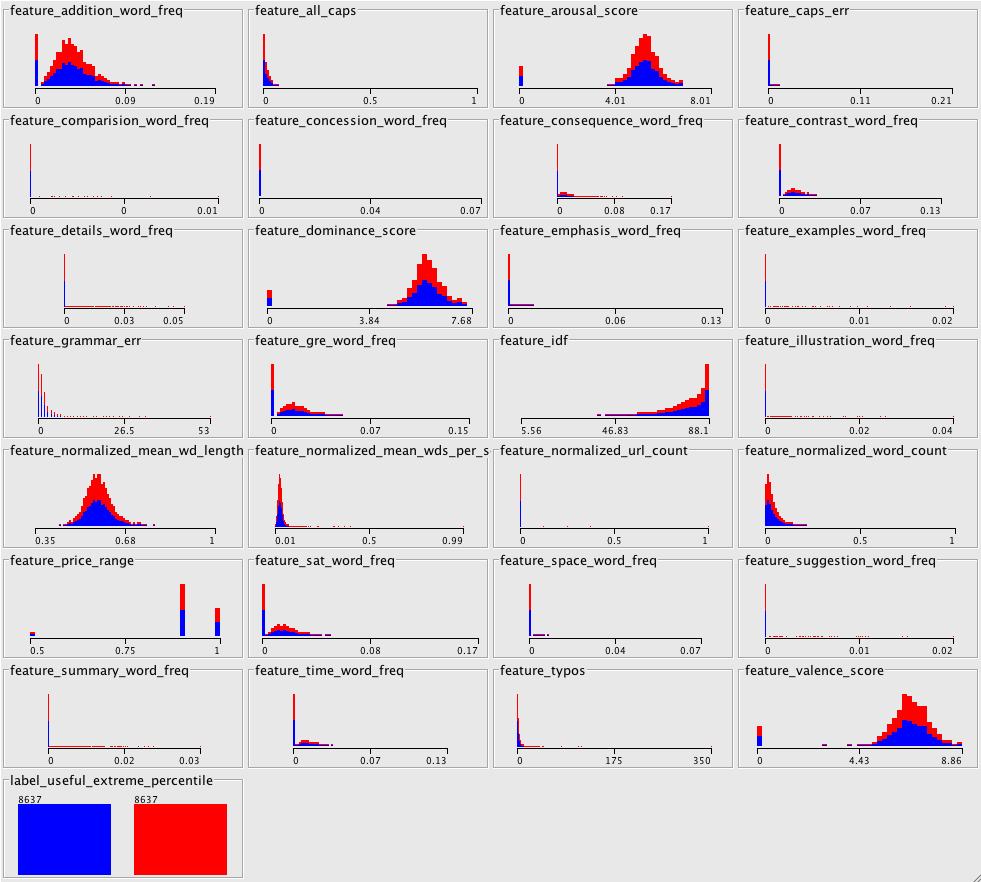
\includegraphics[width=0.75\linewidth]{adaptation_unlabeled_features}
	\caption{Feature distributions for the unlabeled data sets $U_{\textrm{A}}$ and $U_{\textrm{Y}}$.  
	Blue indicates Amazon data feature values and red indicates Yelp feature values.}
\end{figure*}

\subsection{Experiments}
\label{sec:domain-adaptation}

In this set of experiments we use Support Vector Machines to learn
from a combination of both domains; Yelp is considered to be the
\emph{target domain} and Amazon the \emph{source domain}.

We estimate the divergence $\zeta(U_S,U_T)$ as described in the
previous section combining 15,000 examples from each domain.

We performed two sets of experiments. First, we fix the number of
examples from the source domain constant $m_s=2500$, and we vary the
examples from the target distribution $m_t \in \{250, 500, 1000,
2000\}$. Then, we fix $m_t=2500$ constant and we vary $m_s$ in the
same way. 

Figure~\ref{fig:domain-adaptation} shows the results of both
experiments. The left column corresponds to the first experiments where
$m_S$ is fixed; the right column to the experiments where $m_T$ is
fixed. Top row shows a theoretical bound on the error given by
Equation~(\ref{eq:alphaerror}) and the bottom row shows experimental
results.

\begin{figure}
  \centering
  \subfigure[$\zeta(U_S, U_T)=1, m_S=2500$]
  {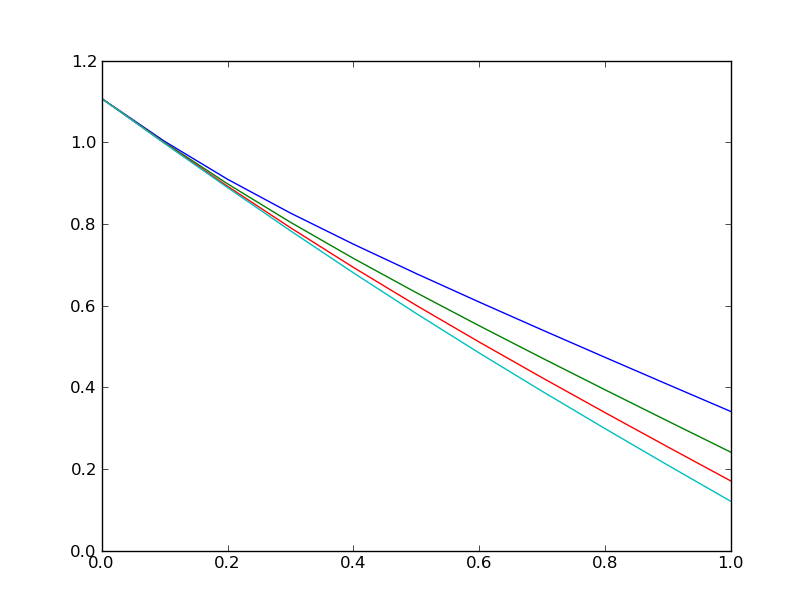
\includegraphics[scale=.3]{adaptation_bound_1_S}}
  \subfigure[$\zeta(U_S, U_T)=1, m_T=2500$]
  {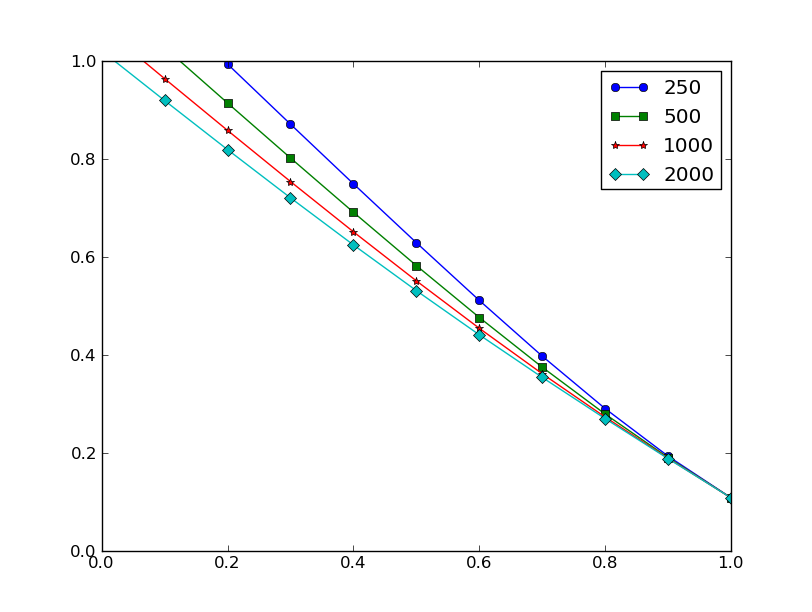
\includegraphics[scale=.3]{adaptation_bound_1_T}}
  \subfigure%[$\zeta(U_S, U_T)=1, m_S=2500$]
  {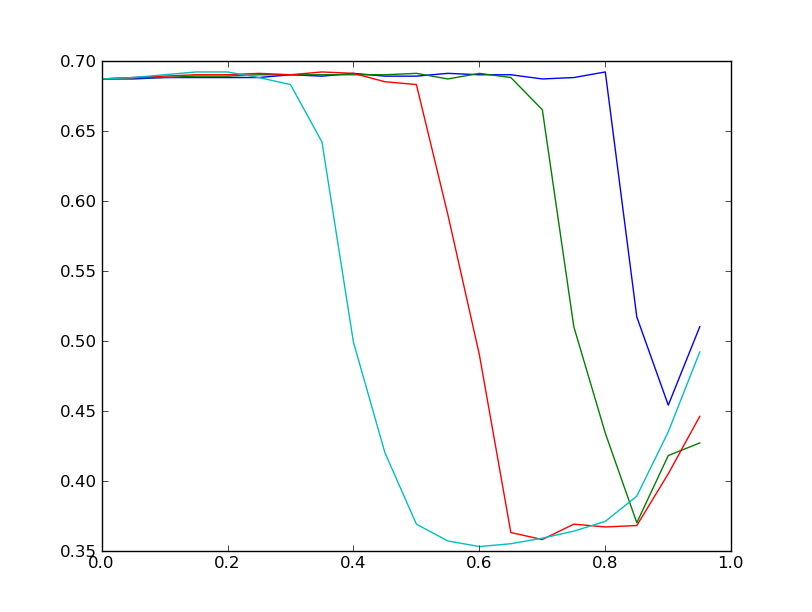
\includegraphics[scale=.3]{adaptation_err_1_S}}
  \subfigure%[$\zeta(U_S, U_T)=1, m_T=2500$]
  {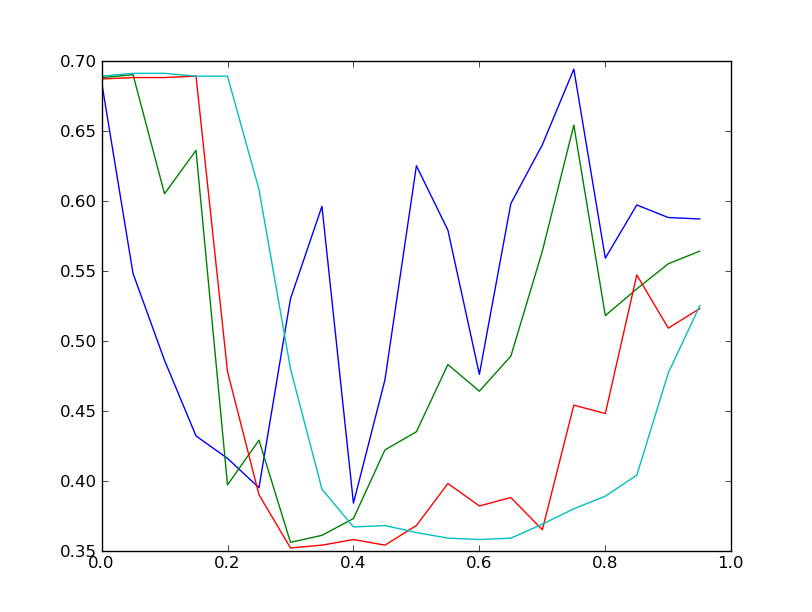
\includegraphics[scale=.3]{adaptation_err_1_T}}
  \caption{Domain adaptation experiments. The $\alpha$-error is shown as a function of $\alpha$ for different combinations of source and target examples.}
  \label{fig:domain-adaptation}
\end{figure}

\section{Future work}
\label{sec:future-work}

Looking at the performances of the algorithms, we observe Adaboost
and linear SVM have similar accuracies on most of the various
experiment instances. As stated in Section \ref{sec:single_domain} one
of the obvious differences is the quality of the confusion matrices. We would like to
investigate the incorrectly classified examples for each algorithm and
come up with an explanation related to what it is minimizing for
classification.  Furthermore, we would like to give a more rigorous explanation on why
Naive Bayes classifier has a dominating accuracy in sparse feature
encoding by comparing the objective functions of our algorithms.

For domain adaptation part, we would like to see how well the classifier
performs when the distance between the target and source distribution
varies keeping the $\beta$ fixed. To alter $\zeta$, we can consider
only a specific category on each domain. 

For example, from the source domain (Amazon), we could consider the
set of categories $C_S$=\{ Books, Electronics, DVDs and Clothing\};
from the target domain (Yelp), we could consider category
$C_T=$\{Restaurants\}. For each combination in $C_s\times C_T$ we
train and test a different linear classifier to estimate the distance
between the two distributions of each configuration.

\section{Conclusion}
\label{sec:conclusion}

In this project, we have used the most popular machine learning
algorithms to determine the quality of a review and we have tried to
apply the notion of domain adaptation to our problem space. One of the
most important remarks is the effect of noise in the data and choice
of the right features for classification. We believe feature extraction
per se can be the most significant factor for the accuracy of the classification and unfortunately we have pursued this part of research rather
intuitively than doing a thorough literature survey. On the other
hand, this has not affected the goal of this project since we have
aimed to look at the nature of the algorithms and domain adaptation
settings. However, we believe its impact on the domain adaptation
experiments is not negligible. 

We have used different machine learning algorithms to determine the
quality of a review using real data from Amazon and Yelp. We have
approached this task as a domain adaptation problem. In particular, we
tried to use a large set of Amazon reviews to predict the quality of
Yelp reviews. One of the most important remarks is the effect of noise
in the data and choice of the right features for classification. We
believe feature extraction per se can be the most significant factor
for the accuracy of the classification. Unfortunately, we have
approached this problem using just intuition rather than a data driven
model or following previous work.  We believe its impact on the domain
adaptation experiments is not negligible. On the other hand, this has
not affected the goal of this project; we have aimed to look at the
nature of the algorithms and the domain adaptation
problem. 


\bibliographystyle{IEEEtran}
\bibliography{bib,IEEEabrv}

\end{document}
